
%	\commit{Jonathan}{05/07}{Swap this part with the previous \newline why we need acceleration before all}

We will first introduce how the time taken by some crucial parts in BWA-MEM makes it a good candidate for acceleration. We will then take a look at GASAL2 architecture to see how it can be integrated in BWA-MEM to accelerate the extension phase of the mapper.


\subsection{BWA-MEM computational parts}

BWA-MEM is a full-featured DNA read mapper based on seed-and-extend. In Chapter 2 we described various processing steps of the mapper. It performs a lot of steps to align a batch of query sequences against a reference genome. The seed-extension part that can be accelerated with GASAL2 represents a considerable amount of fraction of the total time.

We profiled the mapper, by mapping paired-end reads to the the human reference genome "hg19"~\cite{ncbi:hg19}. The read data set consists of two files with 5.2 million sequences each, all of them being 150 bases long. The read data set is SRR949537~\cite{ncbi:srr150} downloaded from Sequence Read Archive. We used 12 threads on our test machine, which will be presented later in Chapter~\ref{chap:measurements}. We reported the time needed for the execution of each thread, then took the mean of all of them. The time share is visible on Figure~\ref{fig:bwatimedivision}. We can see that the extension takes approximately 27\% of the total time. Depending on the data set, this can go from 25\% to 33\%. This makes the extension an interesting part to accelerate, since it takes an reasonable fraction of the total compute time. The measurements also show that a theoretical speed-up of $1/\left(1 - 0.27\right) = 1.37\times$ can be reached by accelerating seed-extension.

\begin{figure}[h!]
	\centering
	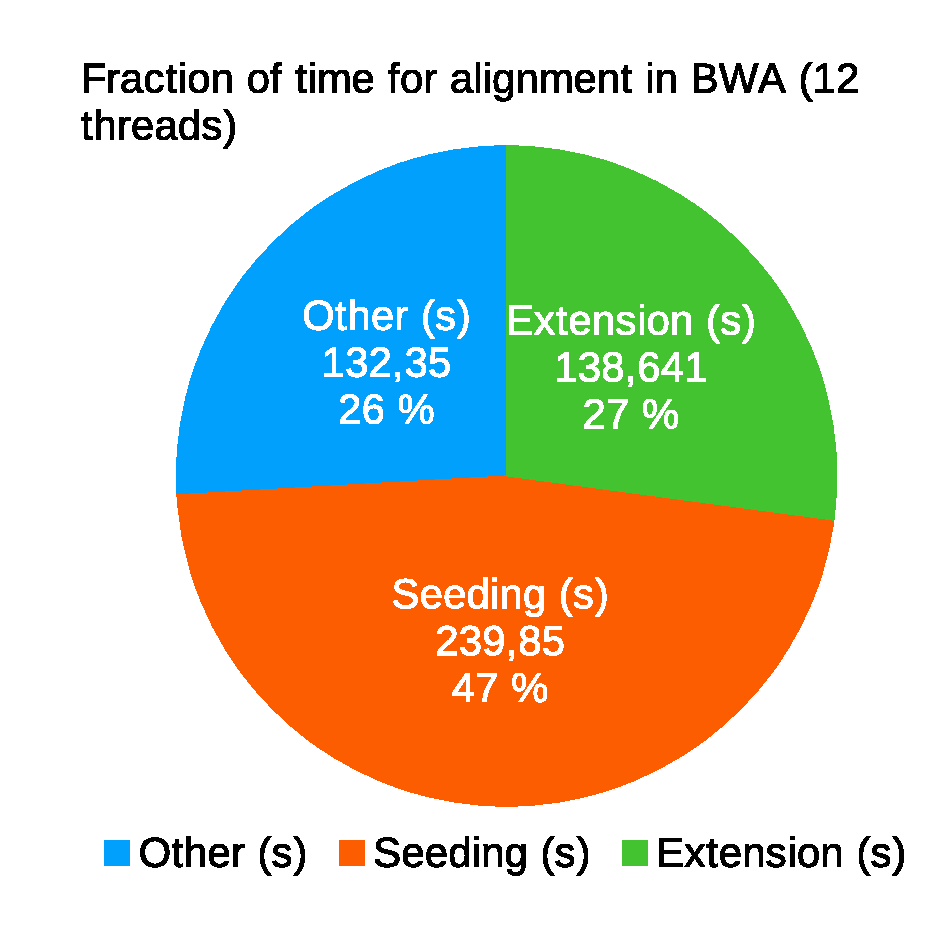
\includegraphics[width=0.65\linewidth]{bwa_time_division}
	\caption{Fraction of time for seeding, extension in an example for BWA.}
	\label{fig:bwatimedivision}
\end{figure}


\subsection{Architecture of GASAL2}
The GASAL2 library is a C++/CUDA library for DNA sequence alignment computation. In the beginning of the project, GASAL2 was able to perform global, local and the semi-global alignment. It features data compression on GPU: the goal is to quickly compress DNA strings directly in VRAM to fetch them faster when calculating the dynamic programming matrix.

Here is the list of features of GASAL2 before this thesis:
\begin{itemize}
	\item Local, global, semi-global sequence alignment run on GPU,
	\item Operates on compressed data: there are 5 bases to describe, A, T, C, G and the unknown base N, hence needing a minimum of 3 bits to encore the base, but each based is stored on 4 bits to facilitate storing (more on this topic below)
	\item Data packing compresses the data directly on GPU: despite having to transfer uncompressed data from host to device, the speed-up provided by parallel processing when packing makes up for the longer transfer time,
	\item Capable to reverse and, or complement any sequence on the batch independently on the GPU.
\end{itemize}

GASAL2 works with batches of sequences to align. Here, we will present the original data structure of GASAL2 . It revolves around a single data structure called \verb|gasal_gpu_storage_t| with the following fields, commented, on Listing~\ref{lst:gpu_storage}. All fields from line 2 to 13 have their counterpart on the GPU, named the same way without the \verb|host_| prefix in their name. Since the host and the device have distinct memories, data should be handed from the host side to the device before launching computation, then the results should be retrieved from the device when it is done.  
These similar fields have been omitted for clarity, and only reminded with the comment \verb|//[copies of the aforementioned field on the GPU]|.

\begin{listing}
	\begin{minted}[
	frame=lines,
	framesep=2mm,
	baselinestretch=1.2,
	fontsize=\footnotesize,
	linenos,
	breaklines,
	frame=single
	]{C}
typedef struct {	
	uint8_t *host_unpacked_query_batch; // (string) the query sequences, butted together
	uint8_t *host_unpacked_target_batch; // (string) the target sequences, butted together
	uint32_t *host_query_batch_offsets; // array with the offsets to tell the sequences apart
	uint32_t *host_target_batch_offsets;
	uint32_t *host_query_batch_lens; // array with the length of each sequence
	uint32_t *host_target_batch_lens;
	
	int32_t *host_aln_score; // array with the alignment scores for all the sequences
	int32_t *host_query_batch_end; // array with the end position of the alignment on the query sequence
	int32_t *host_target_batch_end; // array with the end position of the alignment on the target sequence
	int32_t *host_query_batch_start; // array with the start position of the alignment on the query sequence
	int32_t *host_target_batch_start; // array with the start position of the alignment on the target sequence
	
	//[copies of the aforementioned field on the GPU]
	
	// Information about the batch
	uint32_t gpu_max_query_batch_bytes; // size of the buffer in the GPU (in bytes) for the query sequences
	uint32_t gpu_max_target_batch_bytes; // size of the buffer in the GPU (in bytes) for the target sequences
	uint32_t host_max_query_batch_bytes; // size of the buffer in the host memory (in bytes) for the query sequences
	uint32_t host_max_target_batch_bytes; // size of the buffer in the host memory (in bytes) for the target sequences
	uint32_t gpu_max_n_alns; // maximum number of sequences for the buffers on the GPU
	uint32_t host_max_n_alns; // maximum number of sequences for the buffers on the host
	cudaStream_t str; 
	int is_free; // flag to know if the computation is being run (0) or if it is finished (1)

} gasal_gpu_storage_t;
	\end{minted}
	\caption{the gasal\_gpu\_storage\_t data structure.}
	\label{lst:gpu_storage}
\end{listing}


This structure is initialised for a given size and a number of sequences. Host fields are filled up with the sequences data and their metadata (length, offsets). Trying to fill more than the capacity of the fields results in a forced exit.

GASAL2 went under an important structure rework at the beginning of this thesis to drastically improve its maintainability. In the beginning, it was entirely written in plain C and had a simple architecture consisting in three files:

\begin{itemize}
	\item \verb|gasal.h|: contains all function prototypes and structure definition
	\item \verb|gasal.cu|: contains all functions code and the CUDA calls
	\item \verb|gasal_kernels.h|: contains all CUDA kernels, duplicated
\end{itemize}

Although this may seem as an easy way to split the code, it grew up to the point where it became hardly manageable. The rewrite included separating the different parts of the code in distinct files, adding interfaces for structure filling, and a class to  handle all parameters in an centralized way.

In addition, a shift to C++ has been operated to take advantage of C++ templates: they allow to produce different versions of a given function at compilation time. This will me more discussed on Chapter~\ref{chap:implementation}.

%We can draw an inclusion graph of all the files in GASAL2 in its current form. This graph is shown on Figure~\ref{fig:inclgraph}.

%\commit{Jonathan}{\today}{ADD GRAPH HERE}


